\documentclass{beamer}

% ============================================================
% Colorful Theme Setup
% ============================================================
\usetheme{CambridgeUS}
\usecolortheme{crane}

% Custom vibrant colors
\definecolor{RakutenCrimson}{RGB}{191, 0, 48}
\definecolor{DeepBlue}{RGB}{30, 60, 114}
\definecolor{VividOrange}{RGB}{255, 140, 0}
\definecolor{TealGreen}{RGB}{0, 150, 136}
\definecolor{SoftPurple}{RGB}{123, 63, 228}
\definecolor{LightGold}{RGB}{255, 215, 0}
\definecolor{SoftBg}{RGB}{252, 248, 240}

% Apply Rakuten Crimson as primary color
\setbeamercolor{palette primary}{bg=RakutenCrimson, fg=white}
\setbeamercolor{palette secondary}{bg=DeepBlue, fg=white}
\setbeamercolor{palette tertiary}{bg=RakutenCrimson!80!black, fg=white}
\setbeamercolor{title}{fg=white, bg=RakutenCrimson}
\setbeamercolor{frametitle}{fg=white, bg=RakutenCrimson}
\setbeamercolor{block title}{bg=DeepBlue, fg=white}
\setbeamercolor{block body}{bg=DeepBlue!8, fg=black}
\setbeamercolor{block title alerted}{bg=VividOrange, fg=white}
\setbeamercolor{block body alerted}{bg=VividOrange!8, fg=black}
\setbeamercolor{block title example}{bg=TealGreen, fg=white}
\setbeamercolor{block body example}{bg=TealGreen!8, fg=black}
\setbeamercolor{item}{fg=RakutenCrimson}
\setbeamercolor{subitem}{fg=DeepBlue}
\setbeamercolor{subsubitem}{fg=TealGreen}
\setbeamercolor{section in toc}{fg=RakutenCrimson}

\setbeamertemplate{navigation symbols}{}
\setbeamertemplate{footline}[frame number]
\setbeamerfont{frametitle}{series=\bfseries}

\usepackage{tikz}
\usetikzlibrary{shapes,arrows.meta,positioning,calc,shadows.blur}
\usepackage{amsmath}
\usepackage{graphicx}
\usepackage{fontawesome5}
\usepackage{hyperref}

\title[\textcolor{white}{Internship Report}]{\textbf{Internship Experience Report}}
\subtitle{\textcolor{LightGold}{\textbf{Rakuten India} --- Data Engineering}}
\author{Ankit Kumar Singh \\ 2021IMT-012}
\institute{ABV--IIITM Gwalior}
\date{\today}

\begin{document}

% ============================================================
% SLIDE 1: Title
% ============================================================
\begin{frame}
  \titlepage
\end{frame}

% ============================================================
% SLIDE 2: Outline
% ============================================================
\begin{frame}{Outline}
  \tableofcontents
\end{frame}

% ============================================================
% SLIDE 3: About Rakuten
% ============================================================
\section{About Rakuten}
\begin{frame}[shrink=10]{About Rakuten}
  \begin{columns}[T]
    \begin{column}{0.65\textwidth}
      \begin{itemize}
        \item \textbf{Rakuten Group, Inc.} is a Japanese multinational conglomerate headquartered in Tokyo, founded in 1997 by Hiroshi Mikitani.
        \item One of the \textbf{largest e-commerce and internet companies} globally, operating in \textbf{30+ countries} with \textbf{1.6+ billion members}.
        \item Core businesses span:
        \begin{itemize}
            \item[\textcolor{VividOrange}{\faShoppingCart}] \textbf{E-Commerce}: Rakuten Ichiba, Rakuten Fashion
            \item[\textcolor{TealGreen}{\faCreditCard}] \textbf{Fintech}: Rakuten Card, Rakuten Bank, Rakuten Securities
            \item[\textcolor{SoftPurple}{\faSignal}] \textbf{Mobile \& Telecom}: Rakuten Mobile (4G/5G)
            \item[\textcolor{DeepBlue}{\faCloud}] \textbf{Digital Content}: Rakuten Viber, Rakuten TV
        \end{itemize}
        \item \textbf{Rakuten India}: Engineering hub in Bangalore, focusing on platform engineering, data infrastructure, and AI/ML.
      \end{itemize}
    \end{column}
    \begin{column}{0.3\textwidth}
      \centering
      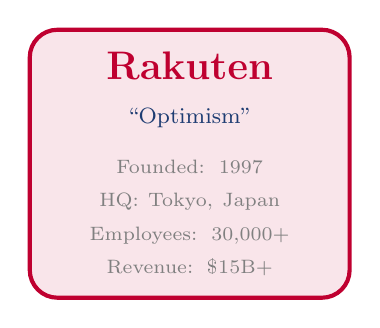
\begin{tikzpicture}
        \node[draw=RakutenCrimson, fill=RakutenCrimson!10, rounded corners=10pt, 
              text width=3.5cm, align=center, inner sep=8pt, line width=1.5pt] {
          {\Large \textcolor{RakutenCrimson}{\textbf{Rakuten}}} \\[4pt]
          {\footnotesize \textcolor{DeepBlue}{``Optimism''}} \\[6pt]
          {\scriptsize \textcolor{gray}{Founded: 1997}} \\
          {\scriptsize \textcolor{gray}{HQ: Tokyo, Japan}} \\
          {\scriptsize \textcolor{gray}{Employees: 30,000+}} \\
          {\scriptsize \textcolor{gray}{Revenue: \$15B+}}
        };
      \end{tikzpicture}
    \end{column}
  \end{columns}
\end{frame}

% ============================================================
% SLIDE 4: My Role
% ============================================================
\section{My Role}
\begin{frame}[shrink=8]{My Role: Data Engineer Intern}
  \begin{block}{\faUserTie\quad Role Overview}
    \textbf{Position}: Data Engineer Intern \\
    \textbf{Team}: Data Platform / Data Engineering \\
    \textbf{Location}: Rakuten India, Bangalore
  \end{block}
  \vspace{0.15cm}
  
  \textbf{Key Responsibilities}:
  \begin{itemize}
    \item[\textcolor{RakutenCrimson}{\faDatabase}] Design and build \textbf{end-to-end data pipelines} (ELT/ETL) for structured and semi-structured data.
    \item[\textcolor{DeepBlue}{\faCogs}] Orchestrate workflows using \textbf{Apache Airflow} for automated scheduling and monitoring.
    \item[\textcolor{TealGreen}{\faCloud}] Work with \textbf{Google Cloud Platform} (GCS, BigQuery, Dataproc) for cloud-native data processing.
    \item[\textcolor{VividOrange}{\faDocker}] Containerize services using \textbf{Docker \& Colima} for reproducible local development on macOS.
    \item[\textcolor{SoftPurple}{\faChartBar}] Ensure data quality, schema validation, and pipeline observability.
  \end{itemize}
  
  \begin{alertblock}{\faStar\quad Tech Stack}
    Python \textbullet{} Apache Airflow \textbullet{} Docker/Colima \textbullet{} GCS \textbullet{} BigQuery \textbullet{} Dataproc (PySpark) \textbullet{} SQL
  \end{alertblock}
\end{frame}

% ============================================================
% SLIDE 5: Project 1 --- Fintech ELT Pipeline
% ============================================================
\section{Projects}
\subsection{Project 1: Fintech ELT Pipeline}
\begin{frame}[shrink=10]{Project 1: End-to-End ELT Pipeline (Fintech Dataset)}
  \begin{exampleblock}{\faProjectDiagram\quad Objective}
    Build a complete \textbf{Extract--Load--Transform (ELT)} pipeline for a fintech dataset, from raw data ingestion through transformation to analytics-ready tables in \textbf{Google BigQuery}.
  \end{exampleblock}
  \vspace{0.2cm}
  
  \textbf{Pipeline Architecture}:
  \begin{center}
  \resizebox{0.95\textwidth}{!}{
  \begin{tikzpicture}[
    node distance=1.8cm,
    stage/.style={rectangle, draw=#1, fill=#1!12, text width=3.2cm, text centered, 
                  rounded corners=8pt, minimum height=2.2cm, font=\small\bfseries,
                  line width=1.2pt, blur shadow={shadow blur steps=5}},
    arrow/.style={-{Stealth[length=8pt]}, line width=2pt, color=#1}
  ]
    \node[stage=VividOrange] (extract) {
      \textcolor{VividOrange}{\faFileDownload} \\[3pt]
      \textbf{Extract} \\[2pt]
      {\scriptsize Raw CSV/JSON} \\
      {\scriptsize Fintech Data}
    };
    \node[stage=DeepBlue, right=of extract] (load) {
      \textcolor{DeepBlue}{\faUpload} \\[3pt]
      \textbf{Load} \\[2pt]
      {\scriptsize Google Cloud} \\
      {\scriptsize Storage (GCS)}
    };
    \node[stage=TealGreen, right=of load] (transform) {
      \textcolor{TealGreen}{\faSyncAlt} \\[3pt]
      \textbf{Transform} \\[2pt]
      {\scriptsize Clean, Validate} \\
      {\scriptsize Schema Enforce}
    };
    \node[stage=SoftPurple, right=of transform] (serve) {
      \textcolor{SoftPurple}{\faChartLine} \\[3pt]
      \textbf{Serve} \\[2pt]
      {\scriptsize BigQuery} \\
      {\scriptsize Partitioned Tables}
    };
    
    \draw[arrow=VividOrange] (extract) -- (load);
    \draw[arrow=DeepBlue] (load) -- (transform);
    \draw[arrow=TealGreen] (transform) -- (serve);
  \end{tikzpicture}
  }
  \end{center}
  
  \vspace{0.1cm}
  \textbf{Key Features}:
  \begin{itemize}
    \item[\textcolor{RakutenCrimson}{\faCheckCircle}] Null handling, special character cleaning, date/time transformation.
    \item[\textcolor{RakutenCrimson}{\faCheckCircle}] Added \texttt{etl\_timestamp} for lineage and \texttt{sales\_yearmonth} for partitioning.
    \item[\textcolor{RakutenCrimson}{\faCheckCircle}] Schema validation before BigQuery load; partitioned by month.
  \end{itemize}
\end{frame}

% ============================================================
% SLIDE 6: Project 2 --- Car Sales Automated Pipeline
% ============================================================
\subsection{Project 2: Car Sales Automated Pipeline}
\begin{frame}[shrink=10]{Project 2: Fully Automated Pipeline (Car Sales Dataset)}
  \begin{exampleblock}{\faRocket\quad Objective}
    Build a \textbf{fully automated, containerized} data pipeline using \textbf{Docker + Colima} on macOS, processing a Car Sales dataset through GCS, Dataproc, and BigQuery with \textbf{dynamic cluster management}.
  \end{exampleblock}
  \vspace{0.2cm}
  
  \textbf{Pipeline Architecture}:
  \begin{center}
  \resizebox{0.95\textwidth}{!}{
  \begin{tikzpicture}[
    node distance=1.2cm,
    stage/.style={rectangle, draw=#1, fill=#1!12, text width=2.6cm, text centered, 
                  rounded corners=6pt, minimum height=1.8cm, font=\scriptsize\bfseries,
                  line width=1pt, blur shadow={shadow blur steps=5}},
    arrow/.style={-{Stealth[length=6pt]}, line width=1.5pt, color=#1}
  ]
    \node[stage=VividOrange] (ingest) {
      \textcolor{VividOrange}{\faFileUpload} \\[2pt]
      \textbf{Ingest} \\[1pt]
      {\tiny Raw CSV} \\
      {\tiny $\rightarrow$ GCS Bucket}
    };
    \node[stage=RakutenCrimson, right=of ingest] (cluster) {
      \textcolor{RakutenCrimson}{\faServer} \\[2pt]
      \textbf{Create Cluster} \\[1pt]
      {\tiny Dataproc} \\
      {\tiny Auto-Scale}
    };
    \node[stage=DeepBlue, right=of cluster] (process) {
      \textcolor{DeepBlue}{\faCogs} \\[2pt]
      \textbf{Process} \\[1pt]
      {\tiny PySpark Job} \\
      {\tiny Transform}
    };
    \node[stage=TealGreen, right=of process] (load) {
      \textcolor{TealGreen}{\faDatabase} \\[2pt]
      \textbf{Load} \\[1pt]
      {\tiny BigQuery} \\
      {\tiny Partitioned}
    };
    \node[stage=SoftPurple, right=of load] (cleanup) {
      \textcolor{SoftPurple}{\faTrashAlt} \\[2pt]
      \textbf{Cleanup} \\[1pt]
      {\tiny Delete Cluster} \\
      {\tiny Cost Saving}
    };
    
    \draw[arrow=VividOrange] (ingest) -- (cluster);
    \draw[arrow=RakutenCrimson] (cluster) -- (process);
    \draw[arrow=DeepBlue] (process) -- (load);
    \draw[arrow=TealGreen] (load) -- (cleanup);
  \end{tikzpicture}
  }
  \end{center}
  
  \vspace{0.1cm}
  \textbf{Key Highlights}:
  \begin{itemize}
    \item[\textcolor{TealGreen}{\faDocker}] Fully \textbf{Dockerized} with Colima (Docker Desktop alternative for macOS).
    \item[\textcolor{DeepBlue}{\faClock}] \textbf{Airflow DAG} orchestrates: Cluster Create $\rightarrow$ PySpark $\rightarrow$ BQ Load $\rightarrow$ Cluster Delete.
    \item[\textcolor{VividOrange}{\faExpandArrowsAlt}] \textbf{Dynamic Dataproc clusters}: Auto-scale workers, created on-demand, deleted after job --- zero idle cost.
    \item[\textcolor{RakutenCrimson}{\faShieldAlt}] GCP IAM, zone-aware provisioning, BigQuery partitioning by \texttt{sales\_yearmonth}.
  \end{itemize}
\end{frame}

% ============================================================
% SLIDE 7: Technical Deep Dive
% ============================================================
\begin{frame}[shrink=8]{Technical Deep Dive: Tools \& Stack}
  \begin{columns}[T]
    \begin{column}{0.48\textwidth}
      \begin{block}{\faLayerGroup\quad Project 1 Stack}
        \begin{itemize}
          \item \textbf{Language}: Python 3.10+
          \item \textbf{Orchestration}: Apache Airflow 2.x
          \item \textbf{Storage}: Google Cloud Storage
          \item \textbf{Warehouse}: BigQuery
          \item \textbf{Data Format}: CSV, JSON
          \item \textbf{Validation}: Custom schema checks
          \item \textbf{Partitioning}: Monthly (\texttt{yearmonth})
        \end{itemize}
      \end{block}
    \end{column}
    \begin{column}{0.48\textwidth}
      \begin{alertblock}{\faLayerGroup\quad Project 2 Stack}
        \begin{itemize}
          \item \textbf{Container}: Docker + Colima
          \item \textbf{Orchestration}: Airflow (Dockerized)
          \item \textbf{Compute}: Dataproc (PySpark)
          \item \textbf{Storage}: GCS Buckets
          \item \textbf{Warehouse}: BigQuery
          \item \textbf{Cluster Mgmt}: Dynamic create/delete
          \item \textbf{Infra}: GCP IAM, Auto-scaling
        \end{itemize}
      \end{alertblock}
    \end{column}
  \end{columns}
  \vspace{0.2cm}
  \begin{center}
    
\begin{tikzpicture}
      \foreach \tool/\clr/\xpos in {Python/VividOrange/0, Airflow/TealGreen/2.2, Docker/DeepBlue/4.4, BigQuery/SoftPurple/6.6, Dataproc/RakutenCrimson/8.8} {
        \node[draw=\clr, fill=\clr!15, rounded corners=5pt, minimum width=1.8cm, minimum height=0.7cm, 
              font=\scriptsize\bfseries, text=\clr!80!black] at (\xpos, 0) {\tool};
      }
    \end{tikzpicture}
  \end{center}
\end{frame}

% ============================================================
% SLIDE 8: Learnings & Takeaways
% ============================================================
\section{Learnings}
\begin{frame}[shrink=10]{Key Learnings \& Takeaways}
  \begin{columns}[T]
    \begin{column}{0.48\textwidth}
      \begin{block}{\faGraduationCap\quad Technical Skills}
        \begin{enumerate}
          \item Designing \textbf{production-grade} ELT/ETL pipelines with proper error handling and logging.
          \item \textbf{Containerization} with Docker/Colima for reproducible environments.
          \item \textbf{Cloud-native} data processing: GCS, BigQuery, Dataproc.
          \item Writing \textbf{PySpark} jobs for distributed data transformation.
          \item \textbf{Airflow DAG} design: dependency management, retries, and monitoring.
        \end{enumerate}
      \end{block}
    \end{column}
    \begin{column}{0.48\textwidth}
      \begin{exampleblock}{\faBriefcase\quad Professional Growth}
        \begin{enumerate}
          \item Working in a \textbf{large-scale} engineering organization with established practices.
          \item Understanding \textbf{cost optimization} in cloud (ephemeral clusters, right-sizing).
          \item \textbf{Data quality} as a first-class concern: schema validation, null handling, type enforcement.
          \item Collaboration using \textbf{Git workflows}, code reviews, and documentation.
          \item Exposure to \textbf{fintech data} compliance and governance requirements.
        \end{enumerate}
      \end{exampleblock}
    \end{column}
  \end{columns}
  \vspace{0.15cm}
  \begin{center}
    \colorbox{RakutenCrimson!10}{\parbox{0.9\textwidth}{\centering
      \textcolor{RakutenCrimson}{\textbf{\faStar\quad Summary}}: Built two end-to-end data pipelines handling real-world datasets, gaining hands-on experience with cloud infrastructure, containerization, and workflow orchestration at production scale.
    }}
  \end{center}
\end{frame}

% ============================================================
% Thank You
% ============================================================
\begin{frame}[plain]
  \begin{tikzpicture}[remember picture, overlay]
    \fill[RakutenCrimson] (current page.north west) rectangle (current page.south east);
    \node[text=white, font=\Huge\bfseries] at (current page.center) {Thank You!};
    \node[text=LightGold, font=\large, below=1.2cm of current page.center] {Questions?};
    \node[text=white!70, font=\small, below=2.5cm of current page.center] {Ankit Kumar Singh \textbullet{} 2021IMT-012 \textbullet{} ABV--IIITM Gwalior};
  \end{tikzpicture}
\end{frame}

\end{document}
